\documentclass{xStandalone}

\begin{document}
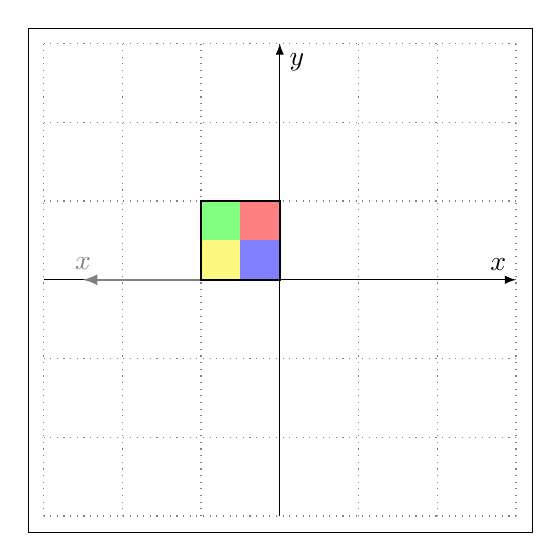
\begin{tikzpicture}

\draw[thin,dotted,gray] (-3,-3) grid[step=1cm] (3,3);

\draw[-latex] (-3,0) -- (3,0) node[above left] {$x$};
\draw[-latex] (0,-3) -- (0,3) node[below right] {$y$};
\draw[-latex,thick,gray] (0,0) -- (-2.5,0) node[above] {$x$};

\fill[blue!50!white]   (0.0,0.0) rectangle (-0.5,0.5);
\fill[yellow!50!white] (-0.5,0.0) rectangle (-1.0,0.5);
\fill[red!50!white]    (-0.0,0.5) rectangle (-0.5,1.0);
\fill[green!50!white]  (-0.5,0.5) rectangle (-1.0,1.0);
\draw[thick] (0,0) rectangle (-1,1);

\draw[ultra thin] (-3.2,-3.2) rectangle (3.2,3.2);



\end{tikzpicture}
\end{document}